\chapter{Μηχανές Διανυσματικής Στήριξης}
\label{appendix:Svm}
Πρόκειται για μία από τις πιο πρόσφατες τεχνικές στον τομέα της επιβλεπόμενης μάθησης, που χρησιμοποιείται ευρέως τόσο σε προβλήματα ταξινόμησης, όσο και σε προβλήματα παλινδρόμησης.
Έστω ότι βρισκόμαστε μπροστά από ένα πρόβλημα ταξινόμησης, με την κλάση να παίρνει 2 τιμές και τα παραδείγματα να έχουν 2 χαρακτηριστικά. Τότε ο χώρος μας είναι κάπως έτσι:
\begin{figure}[H]
	\centering			
%	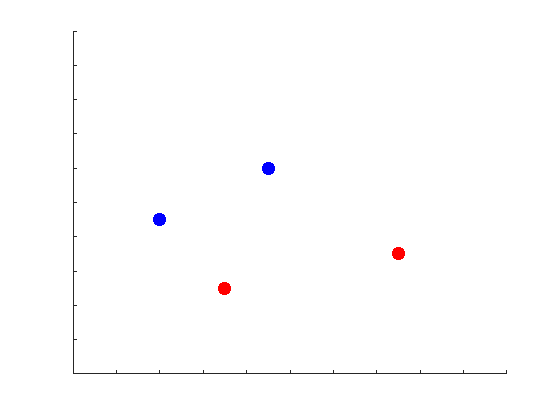
\includegraphics[width=0.6\textwidth, height=6cm]{svm_dots.png}
	\caption[Χώρος ταξινόμησης μηχανής διανυσματικής στήριξης]{Χώρος ταξινόμησης}
\end{figure}
Θα θέλαμε η υπόθεσή μας να διαχωρίσει τα παραπάνω δεδομένα με βάση την κλάση τους, πράγμα που διαπιστώνουμε πως μπορεί να επιτευχθεί με μερικές διαφορετικές υποθέσεις:
\begin{figure}[H]
	\centering
	\begin{minipage}{.333\textwidth}
		\centering
%		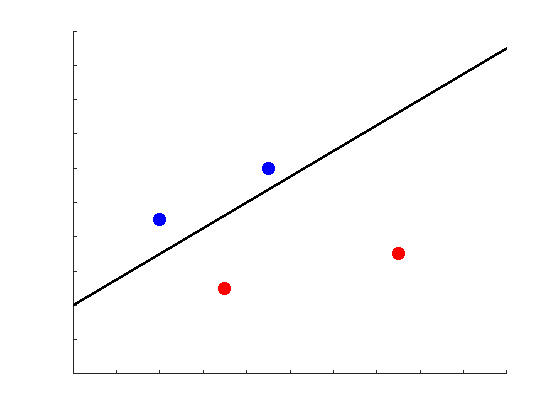
\includegraphics[width=\linewidth, height=0.15\textheight]{svm_line1.png}
		\caption[Υπόθεση Α μηχανής διανυσματικής στήριξης]{Υπόθεση Α}
		
	\end{minipage}%
	\begin{minipage}{0.333\textwidth}
		\centering
%		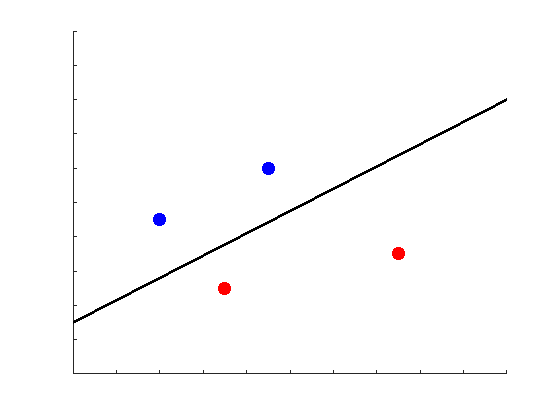
\includegraphics[width=\linewidth, height=0.15\textheight]{svm_line2.png}
		\caption[Υπόθεση Β μηχανής διανυσματικής στήριξης]{Υπόθεση Β}
		
	\end{minipage}
	\begin{minipage}{0.333\textwidth}
		\centering
%		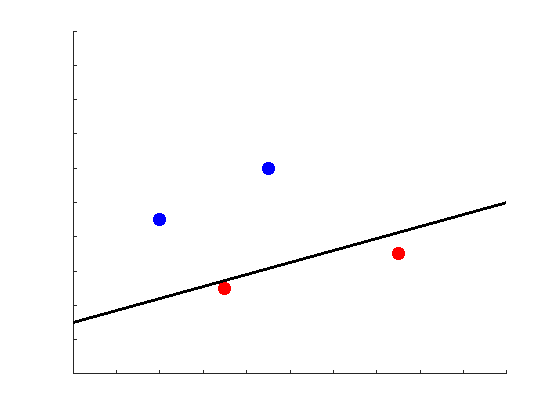
\includegraphics[width=\linewidth, height=0.15\textheight]{svm_line3.png}
		\caption[Υπόθεση Γ μηχανής διανυσματικής στήριξης]{Υπόθεση Γ}
		
	\end{minipage}
\end{figure}
Οι μηχανές διανυσματικής στήριξης μπορούν να απαντήσουν στο εύλογο ερώτημα: ”Ποια από τις παραπάνω υποθέσεις είναι η καλύτερη;” Λαμβάνοντας υπόψιν πως η ποιότητα μιας υπόθεσης καθορίζεται βασικά από την ικανότητά της να γενικεύει, οι αλγόριθμοι αυτοί επιλέγουν την υπόθεση έτσι, ώστε τα πιο κοντινά σημεία που ταξινομούνται σε διαφορετικές κατηγορίες να χωρίζονται από όσο το δυνατόν
μεγαλύτερο κενό. Τα σημεία αυτά ονομάζονται διανύσματα στήριξης. Ένας πιο επίσημος ορισμός, που επεκτείνεται σε περισσότερες διαστάσεις, είναι πως ορίζεται ένα υπερεπίπεδο που διαχωρίζει τις κατηγορίες.

\paragraph{Θεωρητική θεμελίωση} Έστω πως τα δεδομένα μας είναι δισδιάστατα και επιχειρούμε να ορίσουμε την ευθεία που εξασφαλίζει μεγαλύτερο κενό μεταξύ των κοντινότερων σημείων που ανήκουν σε διαφορετική κλάση. Η ευθεία που αναζητούμε φαίνεται στο παρακάτω σχήμα και δίνεται από τον τύπο $w^T x = 0$ και οι ευθείες που περνούν από τα διανύσματα στήριξης ορίζονται ως $w^T x = 1$ και$ w^T x =-1$
\begin{figure}[H]
	\centering			
%	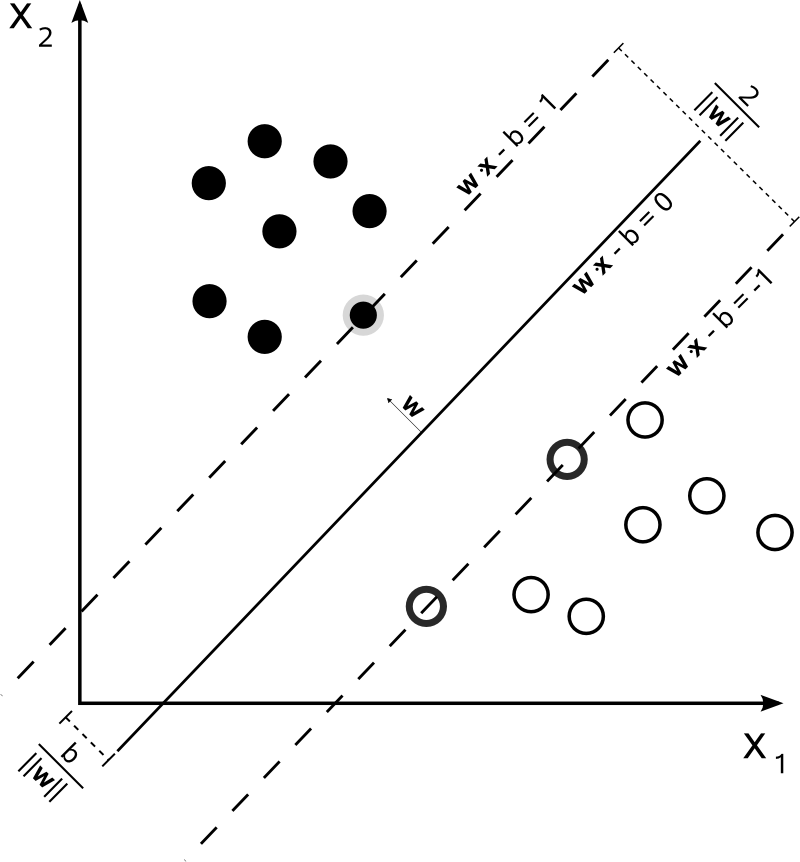
\includegraphics[scale=0.2]{svm.png}
	\caption[Υπερεπίπεδο μηχανών διανυσματικής στήριξης]{Υπερεπίπεδο μηχανών διανυσματικής στήριξης}
\end{figure}
Πριν συνεχίσουμε θα χρειαστεί να ορίσουμε δύο τεχνικές παραδοχές:
\begin{itemize}
	\item Όπως είναι γνωστό, ένα επίπεδο είναι αμετάβλητο ως προς την κλιμάκωση, δηλαδή με όποια σταθερά και να το πολλαπλασιάσω θα συνεχίσω να έχω το ίδιο επίπεδο. Για αυτό θα κανονικοποιούμε ώστε $\norm{w^T x}=1$
	\item  Μας βολεύει να βγάλουμε τον σταθερό όρο $w_0$ από το διάνυσμα w και να ορίσουμε την επιφάνεια ως $w^T  x + b = 0$, όπου προφανώς το b αντιστοιχεί στο $w_0$.
	
\end{itemize}

Πώς υπολογίζουμε την απόσταση ενός σημείου από ένα υπερεπίπεδο;
Αρχικά παρατηρώ πως το w είναι κάθετο στο υπερεπίδεδο. Αυτό αποδεικνύεται πολύ εύκολα ως εξής: Έστω δύο σημεία $x^,$ και $x^{,,}$ πάνω στο υπερεπίπεδο. Τότε ισχύει $w^T  x^, + b = 0$ και $w^T  x^{,,} + b = 0$. Επομένως $w^T (x^, -  x^{,,}) = 0$, δηλαδή το w είναι κάθετο σε οποιαδήποτε ευθεία ενώνει δύο σημεία του υπερεπιπέδου.

Η απόσταση του σημείου $x_n$ από το υπερεπίπεδο υπολογίζεται ως εξής: παίρνω οποιοδήποτε σημείο x στο υπερεπίπεδο και προβάλλω το διάνυσμα $x_n - x$ στο w. Η πράξη αυτή, με το κανονικοποιημένο w να ορίζεται ως $\bar{w}=\frac{w}{\norm{w}}$ , δίνεται από τον τύπο:
$$
distance=\abs{\bar{w} (x_n -x)} =\frac{1}{\norm{w}} \abs{w^T x_n - w^T x}
=\frac{1}{\norm{w}} \abs{w^T x_n  +b - w^T x -b}=\frac{1}{\norm{w}} \\
$$ 
Η προσθαφαίρεση του b μας βοήθησε να παρατηρήσουμε πως το πρώτο άθροισμα ισούται με 1, λόγω της πρώτης παραδοχής, και το δεύτερο άθροισμα δίνει 0, καθώς αποτελεί την εξίσωση του υπερεπιπέδου.

Στη συνέχεια θα προσπαθήσουμε να ορίσουμε το πρόβλημα που προσπαθούν να επιλύσουν οι μηχανές διανυσματικής στήριξης και να το φέρουμε σε τέτοια μορφή, ώστε η επίλυσή του να είναι εύκολη και αυτοματοποιημένη.

Tο πρόβλημα που θέλουμε να βελτιστοποιήσουμε είναι το εξής: θέλουμε να μεγιστοποιήσουμε την απόσταση ενός οποιουδήποτε σημείου από το υπερεπίπεδο υπό τον περιορισμό ότι για το κοντινότερο σημείο, έχουμε κανονικοποιήσει ώστε να ισχύει η εξίσωση $w^T x_n = 1$. Η μαθηματική διατύπωση αυτού του προβλήματος είναι η εξής:
\begin{flalign*}
\text{Μεγιστοποίηση} && \frac{1}{\norm{w}} &&\\
\text{υπό τον περιορισμό ότι} && \min_{n=1,2,...,N} \abs{w^T x + b}=1
\end{flalign*}
Η παραπάνω διατύπωση δεν είναι φιλική προς επίλυση, κυρίως λόγω της μορφής του περιορισμού, για αυτό θα την αναδιατυπώσουμε ως εξής:
\begin{flalign*}
\text{Ελαχιστοποίηση} && \frac{1}{2} w^T w &&\\
\text{υπό τον περιορισμό ότι} && y_n(w^T x_n + b) \geq 1, n=1,...,N
\end{flalign*} 
\\
\fbox{\begin{minipage}{\textwidth}
		\begin{center}
			Πολλαπλασιαστές Lagrange
		\end{center} 
		Πρόκειται για μία μέθοδο εύρεσης τοπικών μεγίστων ή ελαχίστων μιας συνάρτησης που υπακούει σε κάποιον περιορισμό ισότητας. Αν ο σκοπός μου είναι να μεγιστοποιήσω μια συνάρτηση $f(x,y)$ υπό τον περιορισμό ότι $g(x, y) = 0$, τότε αυτή η μέθοδος ορίζει και επιλύει τη συνάρτηση Lagrange $L(x, y, \lambda) = f(x,y) - \lambda g(x,y) $, εισάγοντας μια θετική μεταβλητή χαλαρότητας $\lambda$. Οι προϋποθέσεις Karush–Kuhn–Tucker, επεκτείνουν την εφαρμογή των πολλαπλασιαστών Lagrange,  επιτρέποντας τη βελτιστοποίηση προβλήματα υπό περιορισμούς σε μορφή ανισοτήτων.
	\end{minipage}}
	Η εξίσωση Lagrange, που προκύπτει από το παραπάνω πρόβλημα με τη βοήθεια των προϋποθέσεων Karush–Kuhn–Tucker, είναι η εξής:
	\begin{flalign*}
	\text{Ελαχιστοποίηση} &&L(w,b,a)&= \frac{1}{2} w^T w - \sum_{n=1}^{N} a_n (y_n(w^T x_n +b) -1) &&
	\end{flalign*}
	
	όπου a είναι η θετική μεταβλητή χαλαρότητας που εισήγαγαν οι πολλαπλασιαστές Lagrange.
	Για να ελαχιστοποιήσω ως προς τα w και b, αρκεί να βρω τις μερικές παραγώγους και να τις μηδενίσω:
	\begin{flalign*}
	\text{Άρα} && \nabla_w L &= w-\sum_{n=1}^{N} a_n y_n x_n=0  &&\\
	\text{και} && \frac{\partial L}{\partial b}&= \sum_{n=1}^{N} a_n y_n =0 &&
	\end{flalign*}
	
	Αντικαθιστώντας στην αρχική εξίσωση, το πρόβλημα βελτιστοποίησης διατυπώνεται ως εξής:
	\begin{flalign*}
	\text{Ελαχιστοποίηση} && L(a)= \sum_{n=1}^{N} a_n - \frac{1}{2} \sum_{n=1}^{N} \sum_{m=1}^{N} y_n y_m a_n a_m x_n^T x_m  &&\\
	\text{υπό τη συνθήκη} && \sum_{n=1}^{N} a_n y_n =0 &&\\
	\text{και} && a_n \geq 0  &&
	\end{flalign*}
	\fbox{\begin{minipage}{\textwidth}
			\begin{center}
				Τετραγωνικός Προγραμματισμός
			\end{center} 
			Είναι μια ειδική υποκατηγορία μαθηματικής βελτιστοποίησης, που ασχολείται με τη
			βελτιστοποίηση τετραγωνικών συναρτήσεων μεταβλητών που υπόκεινται σε γραμμικούς περιορισμούς. Στόχος του είναι να βρουν το n-διάστατο διάνυσμα x που ελαχιστοποιεί τη συνάρτηση $\frac{1}{2} x^T Q x + c^T x$ υπό τον περιορισμό $x \leq b$
		\end{minipage}}
		
		Η λύση του παραπάνω προβλήματος δίνεται από κάποιο πακέτο τετραγωνικού περιορισμού, όπου το Q διατυπώνεται ως εξής:
		\[
		\begin{bmatrix}
		y_1y_1x_1^Tx_1 & y_1y_2x_1^Tx_2   & \dots  &  y_1y_Nx_1^Tx_N \\
		y_2y_1x_2^Tx_1 & y_2y_2x_2^Tx_2   & \dots  &  y_2y_Nx_2^Tx_N \\
		\vdots  & \vdots &\ddots & \vdots \\
		y_Ny_1x_N^Tx_ 1& y_Ny_2x_N^Tx_2   & \dots  &  y_Ny_Nx_N^Tx_N \\
		\end{bmatrix}
		\]
		
		Καταφέραμε να διατυπώσουμε το πρόβλημα που επιλύουν οι μηχανές διανυσματικής στήριξης σε όρους προβλήματος βελτιστοποίησης που επιλύεται σχετικά εύκολα. Πρόβλημα θα συναντήσουμε όταν το πλήθος των παρατηρήσεων Ν είναι τόσο μεγάλο ώστε να δίνει στον πίνακα Q απαγορευτικό μέγεθος.
		
		
		\paragraph{Μη γραμμικά διαχωρίσιμες κλάσεις}
		Μέχρι τώρα είδαμε πως οι αλγόριθμοι αυτοί σχηματίζουν υπερεπίπεδα, επομένω κάποιος θα μπορούσε να συμπεράνει πως λειτουργούν μόνο για γραμμικά διαχωρίσιμα προβλήματα. Ωστόσο, αν καταφέρω να μετασχηματίσω τα δεδομένα μου σε κάποιο χώρο μεγαλύτερων διαστάσεων, όπου είναι γραμμικά διαχωρίσιμα, και βρω τα διανύσματα στήριξης εκεί, τότε μπορώ με τον αντίστροφο μετασχηματισμό να βρω τα διανύσματα στήριξης στον αρχικό μου χώρο.
		\begin{figure}[H]
			\centering			
%			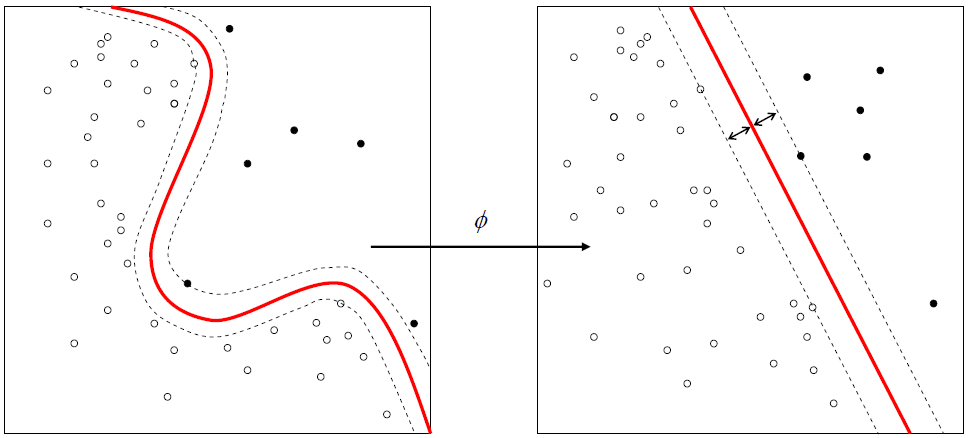
\includegraphics[width=0.8\textwidth, height=6cm]{kernel.png}
			\caption[Χρήση πυρήνα για επίλυση μη γραμμικού διαχωρισμού]{Χρήση πυρήνα για επίλυση μη γραμμικού διαχωρισμού}
		\end{figure}
		
		Έστω πως εκτελώ τον εξής μετασχηματισμό:
		$$X \rightarrow Z$$
		Αν παρατηρήσω την τελική διατύπωση του προβλήματος που επιλύουν αυτοί οι αλγόριθμοι, θα δω πως η μόνη επίδραση αυτού του μετασχηματισμού είναι πως στη θέση των εσωτερικών γινομένων μεταξύ των x, πλέον πρέπει να υπολογίζω εσωτερικά γινόμενα μεταξύ των z σημείων.
		
		Η παραπάνω διαπίστωση μπορεί με μια πρώτη ματιά να μην προκαλεί ενδιαφέρον, αποτέλεσε ωστόσο τον ακρογωνιαίο λίθο στον οποίο βασίζεται η ανωτερότητα αυτής της οικογένειας αλγορίθμων. Ας θεωρήσουμε ένα πρόβλημα ταξινόμησης, όπου τα δεδομένα είναι τόσο περίπλοκα, που προκειμένου να γίνει ο γραμμικός διαχωρισμός τους, να απαιτείται η μεταφορά τους σε κάποιο χώρο τεραστίων, δυνητικά άπειρων διαστάσεων. Εκεί που οι περισσότεροι αλγόριθμοι σηκώνουν τα χέρια ψηλά, οι μηχανές διανυσματικές στήριξης κάνουν την εξής σχεδιαστική επιλογή: αντί να μεταφέρουν τα χαρακτηριστικά σε έναν άπειρο χώρο και να επιλύσουν εκεί το πρόβλημα, ορίζουν μόνο αυτό που χρειάζονται, δηλαδή το εσωτερικό γινόμενο μεταξύ διανυσμάτων στον καινούριο χώρο. Το γινόμενο αυτό αποτελεί μία συνάρτηση που ονομάζεται πυρήνας και συμβολίζεται ως εξής: 
		$$K(x, x^,)= z \cdot z^,$$
		Σε αυτό το σημείο, μπορεί να αναρωτηθεί κάποιος πώς μπορεί να ορίσει έναν πυρήνα, χωρίς να έχει αντίληψη του χώρου, στον οποίο θα μεταφερθεί. Η λογική είναι κάπως ανάποδη: αρκεί να ορίσω μια κάποια συνάρτηση και στη συνέχεια να μπορώ να αποδείξω ότι μπορεί να προκύψει ως εσωτερικό γινόμενο δύο μετασχηματισμένων διανυσμάτων. Υπάρχει μάλιστα η συνθήκη του Mercer, που εξασφαλίζει πως οποιαδήποτε συνάρτηση πυρήνα
		$$K(x, x^,)$$
		είναι έγκυρη, αρκεί να είναι συμμετρική και ο πίνακας που ακολουθεί να είναι θετικά ημιορισμένος:
		\[
		\begin{bmatrix}
		(x_1, x_1) &  (x_1, x_2)  & \dots  &   (x_1, x_N) \\
		(x_2, x_1) &  (x_2 x_2)  & \dots  &   (x_2, x_N) \\
		\vdots  & \vdots &\ddots & \vdots \\
		(x_N, x_1) &  (x_N, x_2)  & \dots  &   (x_N, x_N) \\
		\end{bmatrix}
		\]
		Κατά κανόνα η επιλογή του πυρήνα γίνεται από μια λίστα συχνά χρησιμοποιούμενων συναρτήσεων:
		\begin{itemize}
			\item \textit{Πολυωνυμικός.} Δίνεται από τον τύπο:
			$$K(x, x^,)= (x^T x^, + c)^d$$
			όπου d είναι η διάσταση του νέου χώρου και c μία παράμετρος που καθορίζει την επιρροή που έχουν οι όροι μεγαλύτερης τάξης σε σχέση με τους όρους μικρότερης τάξης.
			\item \textit{Γκαουσιανός (Radial basia function).} Δίνεται από τον τύπο:
			$$K(x, x^,)= e^{(-\frac{\norm{x-x^,}^2}{2 \sigma ^2})}$$
			Ο πυρήνας αυτός μας μεταφέρει σε ένα χώρο άπειρων διαστάσεων. Ο αριθμητής του εκθέτη υπολογίζει την ευκλείδεια απόσταση μεταξύ των 2 σημείων, οπότε μπορούμε να τον αντιληφθούμε ως ένα μέτρο ομοιότητας.
		\end{itemize}
		\paragraph{Μηχανές διανυσματικής στήριξης χαλαρού περιθωρίου}Κάθε φορά λοιπόν που παρατηρούμε μη γραμμικότητα στα δεδομένα μας θα εφαρμόζουμε τη συνάρτηση
		πυρήνα; Ας δούμε το παρακάτω παράδειγμα:
		\begin{figure}[H]
			\centering
			\begin{minipage}{.5\textwidth}
				\centering
%				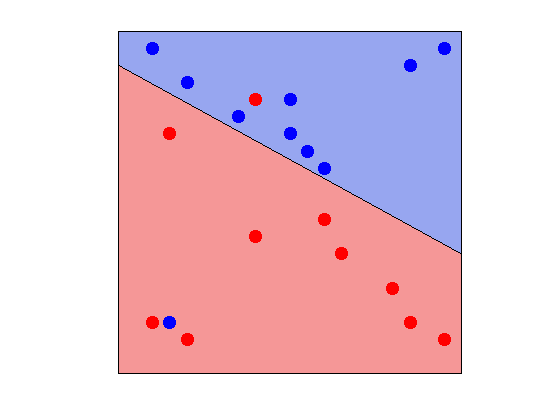
\includegraphics[width=\linewidth, height=0.15\textheight]{soft1.png}
				\caption[Ελάχιστα μη διαχωρίσιμα δεδομένα]{Ελάχιστα μη διαχωρίσιμα δεδομένα}
				
			\end{minipage}%
			\begin{minipage}{0.5\textwidth}
				\centering
%				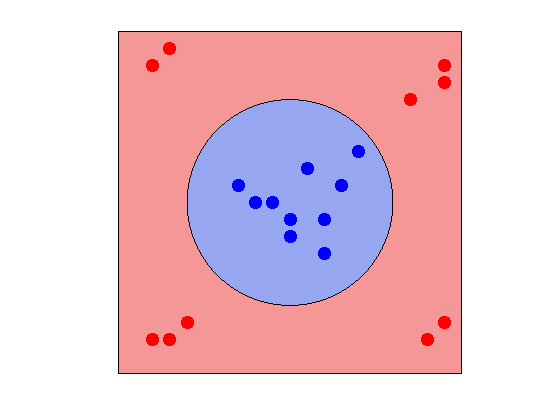
\includegraphics[width=\linewidth, height=0.15\textheight]{soft2.png}
				\caption[Εμφανώς μη διαχωρίσιμα δεδομένα]{Εμφανώς μη διαχωρίσιμα δεδομένα}
				
			\end{minipage}
		\end{figure}
		Και τα δύο σχήματα αντιστοιχούν σε μη γραμμικά διαχωρίσιμα προβλήματα, ωστόσο
		διαφοροποιούνται ποιοτικά: στα αριστερά, ένας γραμμικός διαχωρισμός θα προκαλούσε πολύ μικρό σφάλμα, καθώς μόνο δύο παραδείγματα του σετ εκπαίδευσης θα κατηγοριοποιηθούν λανθασμένα. Αν προσπαθήσω να τα κατατάξω και αυτά σωστά, τότε η υπόθεσή μου θα γίνει πολύ περίπλοκη, καθώς θα χρειαστούν πολλά διανύσματα στήριξης και υποπτεύομαι πως το μοντέλο μου δεν θα γενικεύει. Αντιθέτως, η δεξιά εικόνα αντιστοιχεί σε εμφανώς μη γραμμικά διαχωρίσιμο πρόβλημα, που επιλύεται μόνο με τη χρήση συνάρτησης πυρήνα.
		
		Η απαίτηση δυνατότητας λανθασμένης κατηγοριοποίησης υλοποιείται με μια ειδική κατηγορία των μηχανών διανυσματικής στήριξης: τις μηχανές χαλαρού περιθωρίου. Στους αλγόριθμους αυτούς το υπερεπίπεδο ορίζεται κανονικά, ώστε να μεγιστοποιείται το χάσμα, ωστόσο επιτρέπεται σε κάποια σημεία να το παραβιάσουν, δηλαδή να βρεθούν πέρα από τη νοητή γραμμή του περιθωρίου που ορίζεται από τα διανύσματα στήριξης της κατηγορίας τους.
		
		\begin{figure}[H]
			\centering			
%			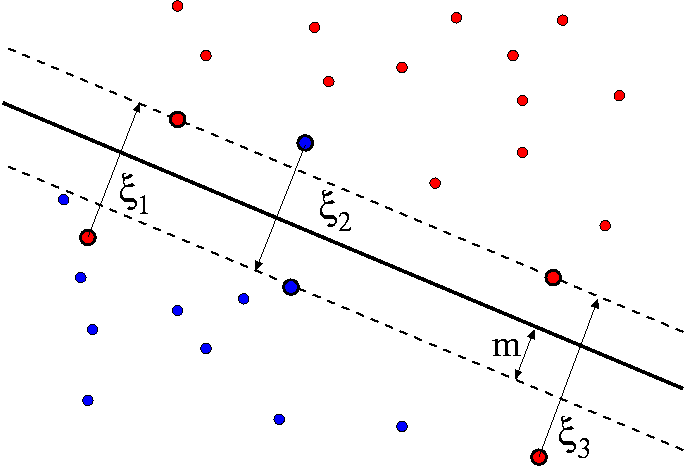
\includegraphics[width=0.8\textwidth, height=6cm]{violation.png}
			\caption[Μηχανές διανυσματικής στήριξης χαλαρού περιθωρίου]{Μηχανές διανυσματικής στήριξης χαλαρού περιθωρίου}
		\end{figure}
		
		Μαθηματικά, οι αλγόριθμοι αυτοί διατυπώνονται ως εξής: Η εξίσωση που ορίζει το περιθώριο εκατέρωθεν του υπερεπιπέδου διαχωρισμού $y_n (w^T x_n + b) \geq 1, n=1,..., N$ πλέον παραβιάζεται, οπότε εισάγουμε μια μεταβλητή χαλαρότητας, την $\xi_n$, ώστε :
		$$y_n (w^T x_n + b) \geq 1 - \xi_n, n=1, ..., N$$
		και η εξίσωση που βελτιστοποιεί πλέον ο αλγόριθμος είναι:
		\begin{flalign*}
		\text{Ελαχιστοποίηση} && \frac{1}{2} w^T w + C \sum_{n=1}^{N} \xi_n  &&\\
		\text{υπό τον περιορισμό ότι} &&y_n (w^T x_n + b) \geq 1 - \xi_n, n=1, ..., N  &&\\
		\text{και} && \xi_n \geq 0  &&
		\end{flalign*}
		Ο παράγοντας C προσδιορίζει πόσο αυστηρός είναι ο αλγόριθμος ως προς τη παραβίαση του περιθωρίου: μία μεγάλη τιμή του C δηλώνει πως επιθυμώ πολύ μικρή παραβίαση.